% !TEX root =  ../main_manuscript.tex 
\section{Personalized Schedule of Invasive Tests for Detecting Progression}
\label{sec:schedule}
We intend to develop a personalized schedule of invasive tests for a new patient $j$, not present in training dataset $\mathcal{A}_n$. Tests are conducted only until \textit{progression} is detected (Figure~\ref{fig:delay_explanation}). Let $T^*_j$ be the true time of progression, and ${t < T^*_j}$ be the time of the latest test on which progression was not detected for the ${j-\mbox{th}}$ patient. Lastly, ${v \geq t}$ denotes the time of the current follow-up visit.

\subsection{Cumulative-risk of progression}
\label{subsec:cum_risk}
First we consolidate history of observed longitudinal outcomes $\{\mathcal{Y}_{1j}(v), \ldots, \mathcal{Y}_{Kj}(v)\}$ until the current visit time $v$, and the previous negative test result ${T^*_j > t}$ into a patient-specific cumulative risk of progression (Figure~\ref{fig:dynrisk_explanation}). It is given by,
\begin{equation}
\label{eq:cumulative_risk}
\begin{split}
R_j(u \mid t, v) &= p\big\{T^*_j \leq u \mid T^*_j > t, \mathcal{Y}_{1j}(v), \ldots, \mathcal{Y}_{Kj}(v), \mathcal{A}_n\big\}\\
&=\int \int p(T^*_j \leq u \mid T^*_j > t, \boldsymbol{b}_{j}, \boldsymbol{\theta}) p\big\{\boldsymbol{b}_j \mid T^*_j > t, \mathcal{Y}_{1j}(v), \ldots, \mathcal{Y}_{Kj}(v), \boldsymbol{\theta} \big\}\\
&\quad \times p(\boldsymbol{\theta} \mid \mathcal{A}_n) \mathrm{d}\boldsymbol{b}_j \mathrm{d}\boldsymbol{\theta}, \quad u \geq t.
\end{split}
\end{equation}
The personalized cumulative-risk function $R_j(\cdot)$ depends on the observed longitudinal data $\{\mathcal{Y}_{1j}(v), \ldots, \mathcal{Y}_{Kj}(v)\}$, and the training dataset $\mathcal{A}_n$ via the posterior distribution of patient-specific random effects~$\boldsymbol{b}_j$, and posterior distribution of the vector of joint model parameters~$\boldsymbol{\theta}$, respectively. The risk also dynamically updates as more longitudinal data becomes available over follow-up (Panel~B~and~C, Figure~\ref{fig:dynrisk_explanation}).

\begin{figure}
\centerline{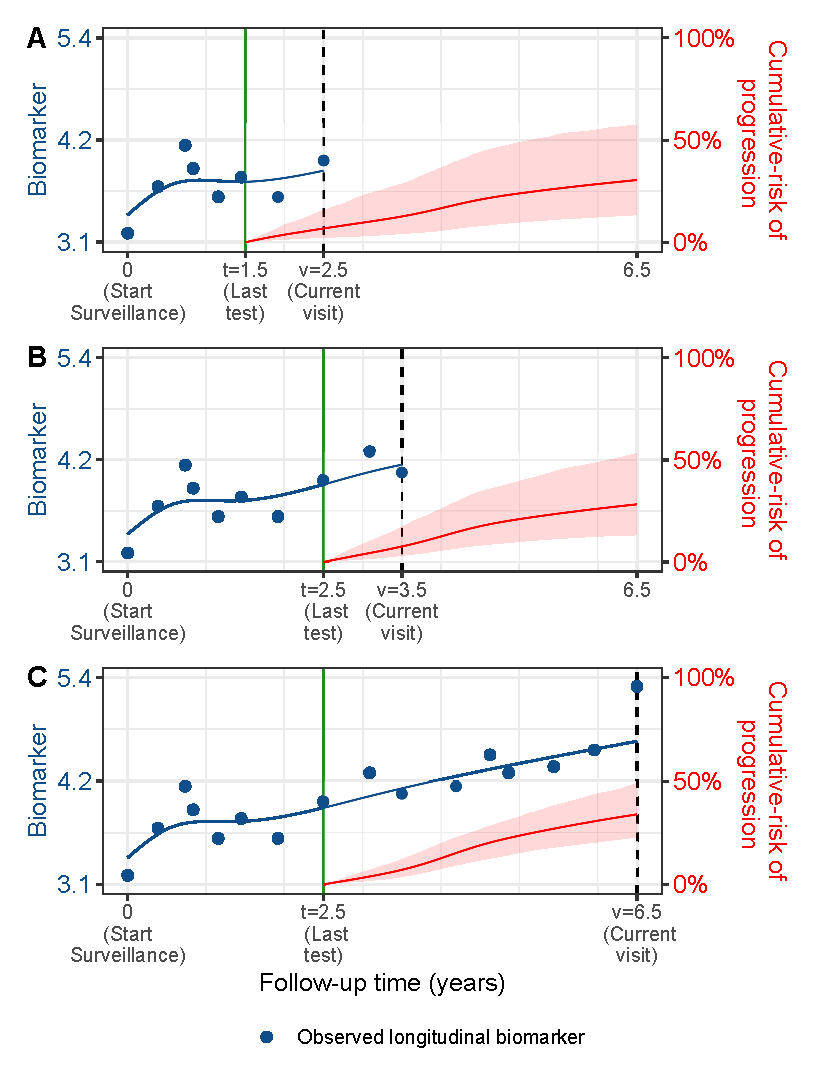
\includegraphics{images/dynrisk_plot_102.eps}}
\caption{\textbf{Cumulative-risk of progression changing dynamically over follow-up} as more patient data is gathered. A single longitudinal outcome, namely, a continuous biomarker of disease progression, is used for illustration. \textbf{Panels~A,~B~and~C:} are ordered by the time of the current visit (dashed vertical black line) of a new patient. At each of these visits, we combine the accumulated longitudinal measurements (shown in blue), and last time of negative invasive test (solid vertical green line) to obtain the updated cumulative risk profile (shown in red) of the patient. All values are illustrative.} 
\label{fig:dynrisk_explanation}
\end{figure}

\subsection{Schedule of Invasive Tests}
Our aim is to employ the cumulative-risk function in Equation~(\ref{eq:cumulative_risk}) to develop a personalized schedule of invasive tests, starting from the current visit time $v$ until a maximum horizon time $h$. For this purpose we utilize a simple and straightforward approach of scheduling invasive tests on all those time points where the conditional cumulative-risk of progression is above a certain threshold $0 \leq \kappa \leq 1$, (e.g., 15\% risk in Figure~\ref{fig:schedule_explanation}). More specifically,
\begin{equation}
\label{eq:personalized_schedule}
\begin{split}
S_j^{\kappa} &= \big\{s_1, \ldots, s_{N} \mid R_j(s_n \mid s_{n-1}, v) = \kappa, s_0 = t \big\}, \quad 1 \leq n \leq N,
\end{split}
\end{equation}
where $s_n$ is the time of the ${n\mbox{-th}}$ test in the personalized test schedule $S_j^{\kappa}$. The conditional cumulative-risk of progression denoted by $R_j(s_n \mid s_{n-1}, v)$ is defined as in Equation~(\ref{eq:cumulative_risk}). It is called `conditional' because each successive ${n\mbox{-th}}$ test at future time $s_{n}$ is scheduled by accounting for the possibility that progression (true time $T^*_j$) may not have occurred until the time of the previously scheduled test $s_{n-1} < T^*_j$. However, the contribution of the observed longitudinal data $\{\mathcal{Y}_{1j}(v), \ldots, \mathcal{Y}_{Kj}(v)\}$ does not change while scheduling subsequent tests. Since the schedule is risk based, it is also updated as more patient data becomes available over follow-up.

\begin{figure}
\centerline{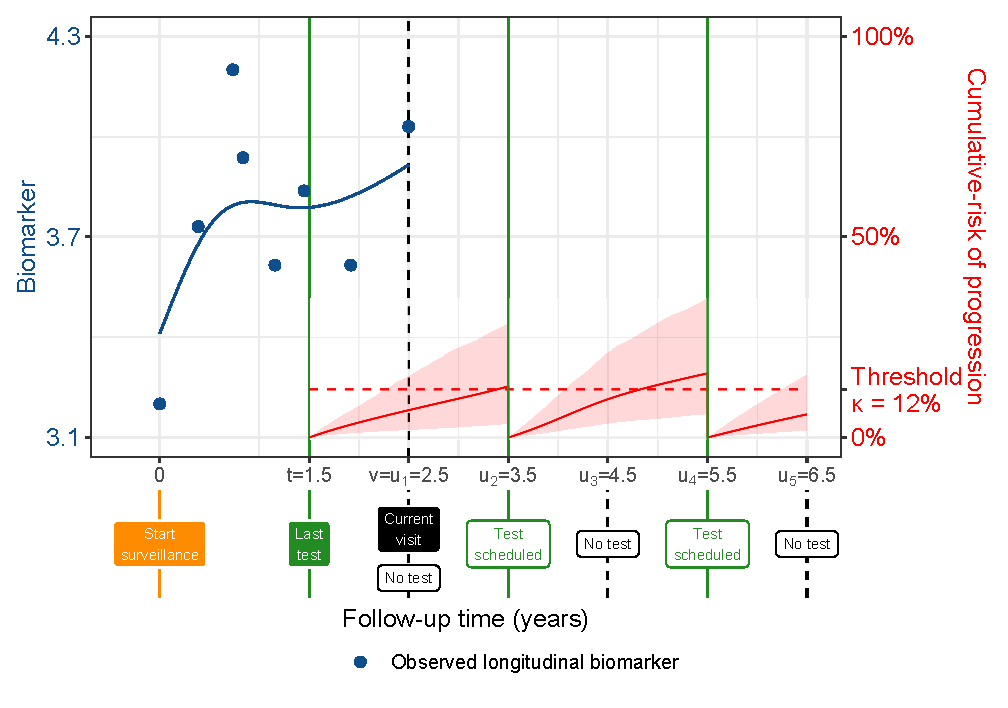
\includegraphics{images/schedule_explanation_102.eps}}
\caption{\textbf{Personalized Invasive Test Schedule Using Patient-specific Conditional Cumulative-risk of Progression}.  A single longitudinal outcome, namely, a continuous biomarker (observed: blue dots, fitted: blue line) of disease progression is used for illustration. The last test on which progression was not observed was conducted at $t=1.5$ years. The current visit time of the patient is $v=2.6$ years. Two future invasive tests are scheduled, $S_j^\kappa = (3.8, 5.7)$ years, using a 15\% risk threshold ($\kappa=0.15$). The conditional cumulative-risk profiles $R_j(s_n \mid s_{n-1}, v)$ of Equation~(\ref{eq:personalized_schedule}) are shown with red line (confidence interval shaded). It is called `conditional' because, for example, the second test at future time 5.7 years, is scheduled after accounting for the possibility that progression (true time $T^*_j$) may not have occurred until the time of the previously scheduled test at $3.8 < T^*_j$ years. All values are illustrative.} 
\label{fig:schedule_explanation}
\end{figure}

\subsection{Risk Threshold $\kappa$}
The risk threshold $\kappa$ controls the timing and the total number of invasive tests in the schedule $S_j^{\kappa}$. Through the timing of tests, $\kappa$ also indirectly affects the time delay (Figure~\ref{fig:delay_explanation}) that may occur in the detection of progression if this schedule is followed. Hence, $\kappa$ should be chosen while balancing both the number of invasive tests (burden), and the time delay in the detection of progression (less is beneficial).

Consider the bi-dimensional Euclidean space of the total number of invasive tests (x-axis) and the corresponding expected time delay in detection of progression (y-axis) for schedules associated with various $\kappa$ (Figure~\ref{fig:kappa_choice}). An ideal schedule of tests will have only one test planned exactly at the true time of progression $T^*_j$ of a patient. In other words it will lead to a zero time delay. This schedule is shown at the point of optimality (1, 0) in Figure~\ref{fig:kappa_choice}. Subsequently, a threshold $\kappa_a$ can be chosen automatically by minimizing the Euclidean distance between the point $(1,~0)$ and the set of points representing various schedules corresponding to each $0 \leq \kappa \leq 1$. That is,
\begin{equation}
\label{eq:kappa_choice}
\kappa_a = \argmin_{\kappa} \sqrt{\big(\vert S_j^\kappa \vert - 1\big)^2 + \big\{D_j(S_j^{\kappa} \mid t, v) - 0\big\}^2} , \quad 0 \leq \kappa \leq 1,
\end{equation}
where, $D_j(S_j^{\kappa} \mid t, v)$ denotes the expected time delay in detection of progression (estimation in Section~\ref{subsec:exp_delay_estimation}) if schedule $S_j^{\kappa}$ is followed. Additional consequences of following a particular schedule, such as life years saved, or quality-adjusted life years saved, can also be accommodated in Equation~(\ref{eq:kappa_choice}). However, this first requires setting a point of optimality in a higher dimensional Euclidean space of the aforementioned consequences.

Certain patients may have preferences for the maximum number of invasive tests conducted upon them. Others may be apprehensive about having an expected time delay higher than a certain number of months. In this regard, the Euclidean distance in Equation~(\ref{eq:kappa_choice}) can be minimized under constraints on the number of tests or delay (Figure~\ref{fig:kappa_choice}). An additional benefit of this approach is that it alleviates the issue of time delay and the number of tests having different units of measurement~\citep{cook1994equivalence}.

\begin{figure}
\centerline{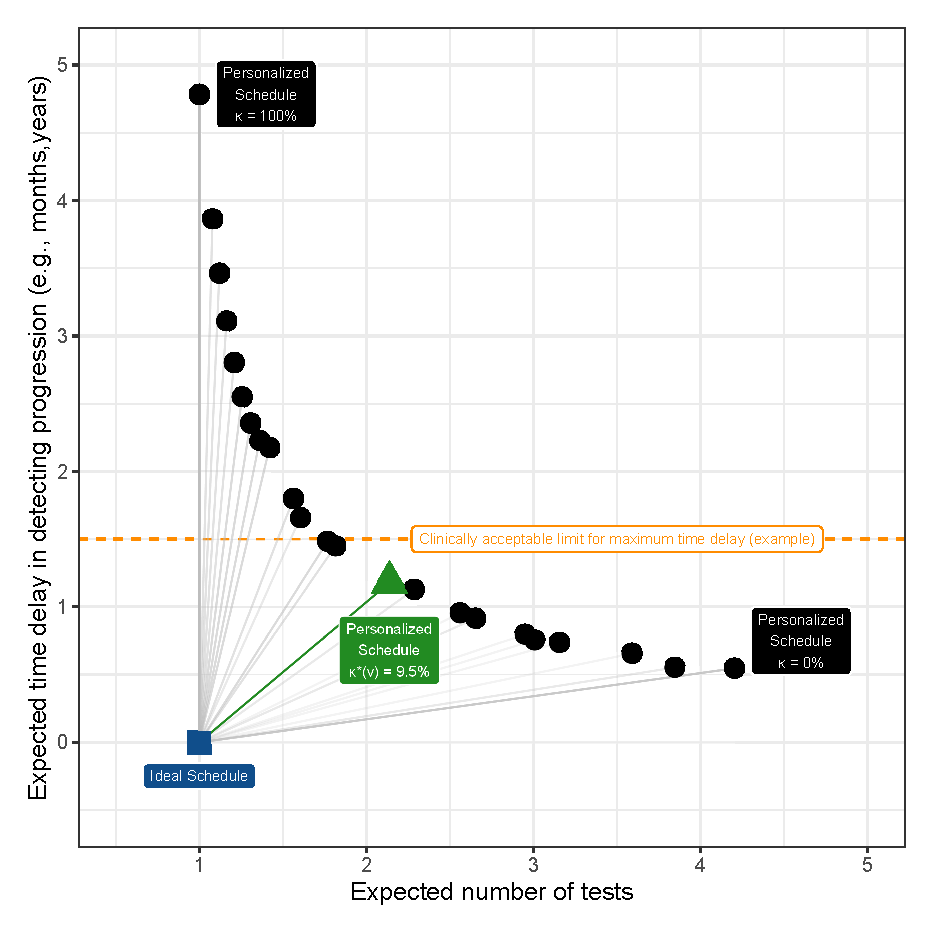
\includegraphics{images/kappa_choice_102.eps}}
\caption{\textbf{Automatic choice of risk threshold $0 \leq \kappa \leq 1$ using Equation~(\ref{eq:kappa_choice})}. The ideal schedule of tests at point (1,0) is shown as a blue square. It plans exactly one biopsy at the true time of progression $T^*_j$ of a patient and hence leads to a zero time delay in detection of progression. Personalized schedules based on a grid of thresholds chosen between $0 \leq \kappa \leq 1$ are shown with black circles. Higher thresholds lead to fewer biopsies, but also higher expected time delay. We propose to choose the personalized schedule based on $\kappa_a=21.2\%$ threshold (green triangle). This is because it has the least Euclidean distance (shown with a green line) to the ideal schedule. It is also possible to find the least distance under a certain clinically acceptable threshold on time delay (orange dashed line), or number of biopsies.}
\label{fig:kappa_choice}
\end{figure}

\subsection{Expected Time Delay in Detection of Progression}
\label{subsec:exp_delay_estimation}
We estimate the expected time delay $D_j(S_j^{\kappa} \mid t, v)$ in Equation~\ref{eq:kappa_choice} in a patient-specific manner as well. That is, two patients may opt to follow the same schedule, but they will expect different time delays. To this end, we utilize the personalized cumulative-risk profile estimated in Equation~(\ref{eq:cumulative_risk}). Furthermore, the calculation of time delay is not limited to personalized schedules (Equation~\ref{eq:personalized_schedule}) only. Rather, for any schedule $S$ of $N$ invasive tests, the personalized expected delay for the ${j\mbox{-th}}$ patient is given by,
\begin{equation}
\label{eq:expected_delay}
\begin{split}
D_j(S \mid t, v) &= \sum_{n=1}^{N} R_j(s_n \mid s_{n-1}, v) d_j(s_n, s_{n-1}, v), \quad s_0 = t\\
d_j(s_n, s_{n-1}, v) &= s_n - s_{n-1} - E(T^*_j \mid s_{n-1}, s_n, v),\\
E(T^*_j \mid s_{n-1}, s_n, v) &= \int_{s_{n-1}}^{s_n} p\Big\{T^*_j \geq u \mid s_{n-1} < T^*_j \leq s_n, \mathcal{Y}_{1j}(v), \ldots, \mathcal{Y}_{Kj}(v), \mathcal{A}_n\Big\} \mathrm{d}u,
\end{split}
\end{equation}
where $s_n$ is the time of the ${n\mbox{-th}}$ invasive test in schedule $S$, and ${E(T^*_j \mid s_{n-1}, s_n, v)}$ is the conditional expected progression time, given that the patient obtains progression between the two consecutive tests conducted at times $s_{n-1}$ and $s_n$. This expected progression time is used to calculate individual time delays $d_j(s_n, s_{n-1}, v)$, under the scenario that patient obtains progression in the time interval $s_{n-1} < T^*_j \leq s_n$. Subsequently, we obtain the overall personalized expected time delay $D_j(S \mid t, v)$ as a weighted average of the individual delays $d_j(s_n, s_{n-1}, v)$. Hence, the personalized expected time delay $D_j(S \mid t, v)$ should be interpreted as the delay if $T^*_j \leq s_N$. That is, if the patient obtains progression before the last invasive test in the schedule $S$. Personalized expected delay can assist patients and doctors in shared decision making of an appropriate biopsy schedule. Although, in order to have a fair comparison of expected delay between different schedules for the same patient, a compulsory test at a common horizon time point should be planned in all schedules.